\chapter{Organization Essence Revealing}

The goals of this chapter are to perform an OER analysis as described in~\cite{dietz2015teoo,dietz2020enterprise}. For simplicity, we will only do the following steps: 

\begin{enumerate}
    \item Insert the project domain description into this document. 
    \item Perform the OER analysis and find \oact{ontological acts}. Be vigilant about the \btrap{blue traps}!
    \item Identify ontological transaction kinds and put them in the text. E.g. \oact{[TK1/rq]} If there are not enough red transactions, you can include the green ones. 
    \item Create an extended transaction result table (e-TRT). Map the transaction acts to the project domain description. See the~\cref{tab:etrt}. 
    \item Create a Subject-Actor table to realize the distinction between roles and DEMO actor roles. See the~\cref{tab:subjectactortable}. 
    \item Think in trees, not in flows and create the interaction structure of your transaction kinds. See the~\cref{fig:interactionStructure}.  
    \item Produce the Coordination Structure Diagram (CSD) and the Object Fact Diagram (OFD). See the~\cref{fig:csdModel} and ~\cref{fig:ofdModel}.  
    \item Finally, summarize your modeling thoughts and revelations. Don't forget about missing transaction steps table~\cref{tab:missing_transaction_steps}. 
\end{enumerate}

The process description of the Volley Case and it's OER analysis was taken from the Enterprise Ontology book~\cite{dietz2020enterprise}. 

%In the step 1 a coloring of the process description is made. The coloring can be done on text as well as on the flow chart diagram. 
\section{OER Step 1: Distinguishing Performa-Informa-Forma}

Legend: 
\begin{itemize}
    \item \oact{Ontological Act [Transaction Kind/Act type]}
    \item \btrap{Blue trap ontological act}!
\end{itemize}

\paragraph{\S 1 Preliminary Rules}

\begin{enumerate}[label={(\arabic*)}]
\item One can \oact{become member of the tennis club Volley[TK1]} by \btrap{sending a letter}\oact{[TK1/rq]} to the club by postal mail. In the letter one has to mention \iact{one’s surname and first name, birth date, gender, telephone number, and postal mail address (street, house number, zip code, and town)}. Adam, the administrator of Volley, \dact{empties the mailbox} daily and checks whether the information provided is complete. If not, he \dact{makes a telephone call} to the sender in order \iact{to complete the data}. Once a letter is complete, Adam \dact{writes an incoming mail number and the date on the letter, records the letter in the letter book, and puts it in a folder}. 
\item Every Wednesday evening, Adam \dact{takes the folder} to Eve, the secretary of Volley. He also \dact{takes the member register with him}. If Eve \oact{decides that an applicant can become member of Volley[TK1/pm]}, \dact{she stamps ‘new member’ on the letter and writes the date below it. She then hands the letter to Adam in order to add the new member to the member register. This is a book with numbered lines. Each new member is entered on a new line. The line number is the number by which the new member is referenced in the administration}. Next, Eve \iact{calculates the fee} that the new member \oact{has to pay [TK2]} for the remaining part of the calendar year. She asks Adam for the \iact{annual fee}, as \oact{decided at the general assembly [TK out of scope]}, which Adam \dact{has recorded on a sheet of paper}. Then, she asks Adam to \dact{write down the amount in the member register}. 
\item If Eve \oact{does not allow an applicant to become member[TK1/dc]} (e.g. because he or she is too young or because the maximum number of members has been reached), Adam will \btrap{send a letter}\oact{[TK2/rq]} in which he \iact{explains why the applicant cannot (yet) become member of Volley}.
\end{enumerate}

\paragraph{\S 2 Some Other Rules}

\begin{enumerate}[label={(\arabic*)}]
\item When all applications are processed, Adam \dact{takes the letters and the member register home} and \iact{prepares an invoice} to all new members for the \oact{payment of the first fee[TK2]}. He \btrap{sends these invoices}\oact{[TK2/rq]} \dact{by postal mail}. Payments have to be performed by bank transfers.
\item As soon as \btrap{a bank statement is received}\oact{[TK2/da]}, Adam \dact{prints a card} on which \iact{the member number, the starting date, the name, the date of birth, the gender, and the residence} are mentioned. \btrap{The card is sent}\oact{[TK1/da]} \dact{to the new member by postal mail}.
\end{enumerate}





\begin{landscape}
\section{OER Step 2: Identifying Transaction Kinds and Actor Roles}

\begin{table}[h]
\caption{Extended Transaction Result Table}
\label{tab:etrt}
\begin{tabular}{|l||l|l|}
\hline
Transaction  & Issuing judgement by acknowledgement (TK1) & Issuing judgement for default (TK2) \\ \hline
Product      & Judgement by acknowledgement has been issued  & Judgement for default has been issued \\ \hline
Initiator      &  (AR1)   &  (AR2)\\ \hline
Executor       &  (AR2) &  (AR3)       \\ \hline
Request        & TODO (\S1/1)  & TODO (\S2/1)   \\ \hline
Promise        & TODO (\S1/2)  &  Not Specified (Probably Tacit)   \\ \hline
Decline        &  TODO (\S1/3)  & Not Specified  \\ \hline
Declare        & TODO (\S2/2) & A bank statement is received  (\S2/2) \\ \hline
Reject         &  Not Specified             &  Not Specified   \\ \hline
Accept         & Not Specified (Probably Tacit) &  Not Specified (Probably Tacit) \\ \hline
Revoke Request & Not Specified                   & Not Specified        \\ \hline
Revoke Promise & Not Specified                   &  Not Specified       \\ \hline
Revoke Declare & Not Specified                    &  Not Specified      \\ \hline
Revoke Accept  &  Not Specified             &   Not Specified             \\ \hline
\end{tabular}
\end{table}

\begin{table}[h]
\caption{Extended Transaction Result Table}
\label{tab:etrt}
\begin{tabular}{|l||l|l|}
\hline
Transaction  & Annuling judgement for default (TKš) & Correcting the reasoning of the judgment (TK4) \\ \hline
Product      & Judgement for default has been anulated  & Reasoning of the judgement has been corrected \\ \hline
Initiator      &  TODO   &  TODO\\ \hline
Executor       &  TODO &  TODO       \\ \hline
Request        & TODO(\S1/1)  & May propose correcting the reasoning before the judgment becomes final.  (\S165/1)   \\ \hline
Promise        &  TODO  (\S1/2)  &  Not Specified (Probably Tacit)   \\ \hline
Decline        &  The court may not comply. (\S1/3)  & Not Specified  \\ \hline
Declare        & TODO (\S2/2) & TODO (\S2/2) \\ \hline
Reject         &  Not Specified             &  Not Specified   \\ \hline
Accept         & Not Specified (Probably Tacit) &  Not Specified (Probably Tacit) \\ \hline
Revoke Request & Not Specified                   & Not Specified        \\ \hline
Revoke Promise & Not Specified                   &  Not Specified       \\ \hline
Revoke Declare & Not Specified                    &  Not Specified      \\ \hline
Revoke Accept  &  Not Specified             &   Not Specified             \\ \hline
\end{tabular}
\end{table}

\begin{table}[h]
\caption{Extended Transaction Result Table}
\label{tab:etrt}
\begin{tabular}{|l||l|l|}
\hline
Transaction  & Correcting the reasoning of the judgment by court of appeal  (TK5) &  (TK6) \\ \hline
Product      & The reasoning of the judgement has been corrected by court of appeal  & TODO \\ \hline
Initiator      &  TODO   &  TODO\\ \hline
Executor       &  TODO &  TODO       \\ \hline
Request        & Makes proposal to correct the reasoning of the judgment (\S165/2)  & TODO  \\ \hline
Promise        &  TODO  (\S1/2)  &  Not Specified (Probably Tacit)   \\ \hline
Decline        &  The court may not comply. (\S1/3)  & Not Specified  \\ \hline
Declare        & TODO (\S2/2) & TODO (\S2/2) \\ \hline
Reject         &  Not Specified             &  Not Specified   \\ \hline
Accept         & Not Specified (Probably Tacit) &  Not Specified (Probably Tacit) \\ \hline
Revoke Request & Not Specified                   & Not Specified        \\ \hline
Revoke Promise & Not Specified                   &  Not Specified       \\ \hline
Revoke Declare & Not Specified                    &  Not Specified      \\ \hline
Revoke Accept  &  Not Specified             &   Not Specified             \\ \hline
\end{tabular}
\end{table}

\begin{table}[h]
\caption{Subject Actor Table}
\label{tab:subjectactortable}
\begin{tabular}{|l|l|l|l|l|}
\hline
  & (AR1)  &  (AR2)  &  (AR3) & (AR4)  \\ \hline
Defendant & X  &  &  &  \\ \hline
Court &  & X &  & X \\ \hline
Plaintiff &  &  & X & \\ \hline


\end{tabular}
\end{table}

\end{landscape}

\section{OER Step 3: Composing the Essential Model}

Before starting with a CSD model, it is important to think about the transaction interaction structure. The transaction have to form one or more trees to compose into a process. You can see an example in~\cref{fig:interactionStructure}. 

\begin{figure}[h]\centering
	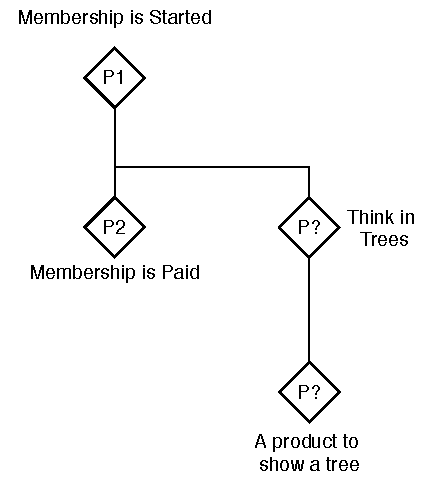
\includegraphics[width=8cm]{pic/VolleyInteractionStructure}
	\caption{An Interaction Structure Model of Volley}
	\label{fig:interactionStructure}
\end{figure}

\begin{figure}[h]\centering
	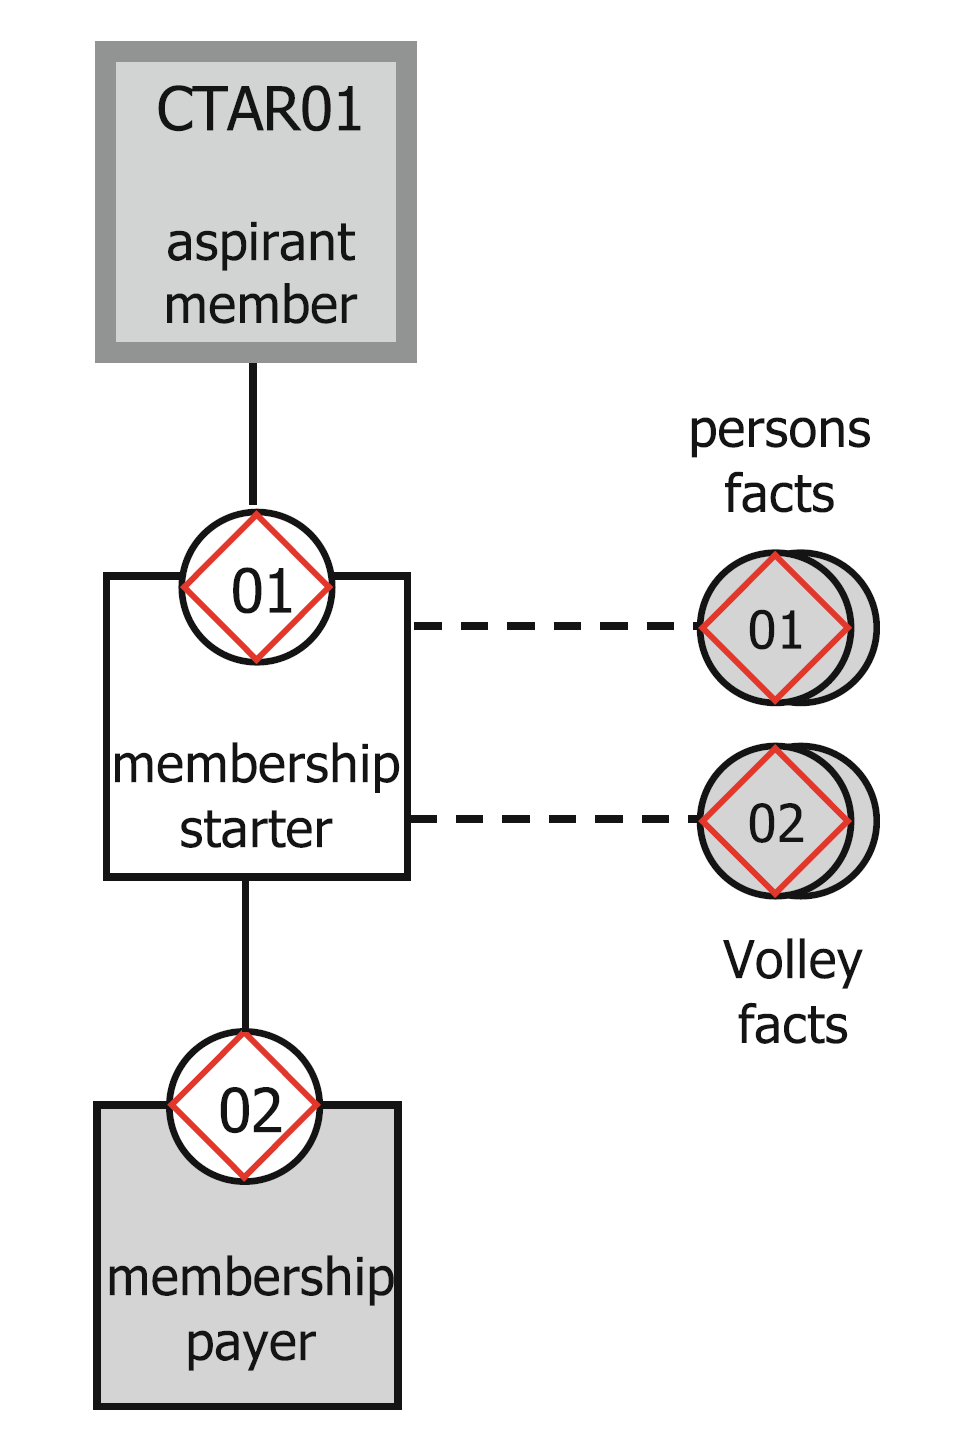
\includegraphics[width=6cm]{pic/VolleyCSD}
	\caption{A CSD Model of Volley~\cite{dietz2020enterprise}}
	\label{fig:csdModel}
\end{figure}

\begin{figure}[h]\centering
	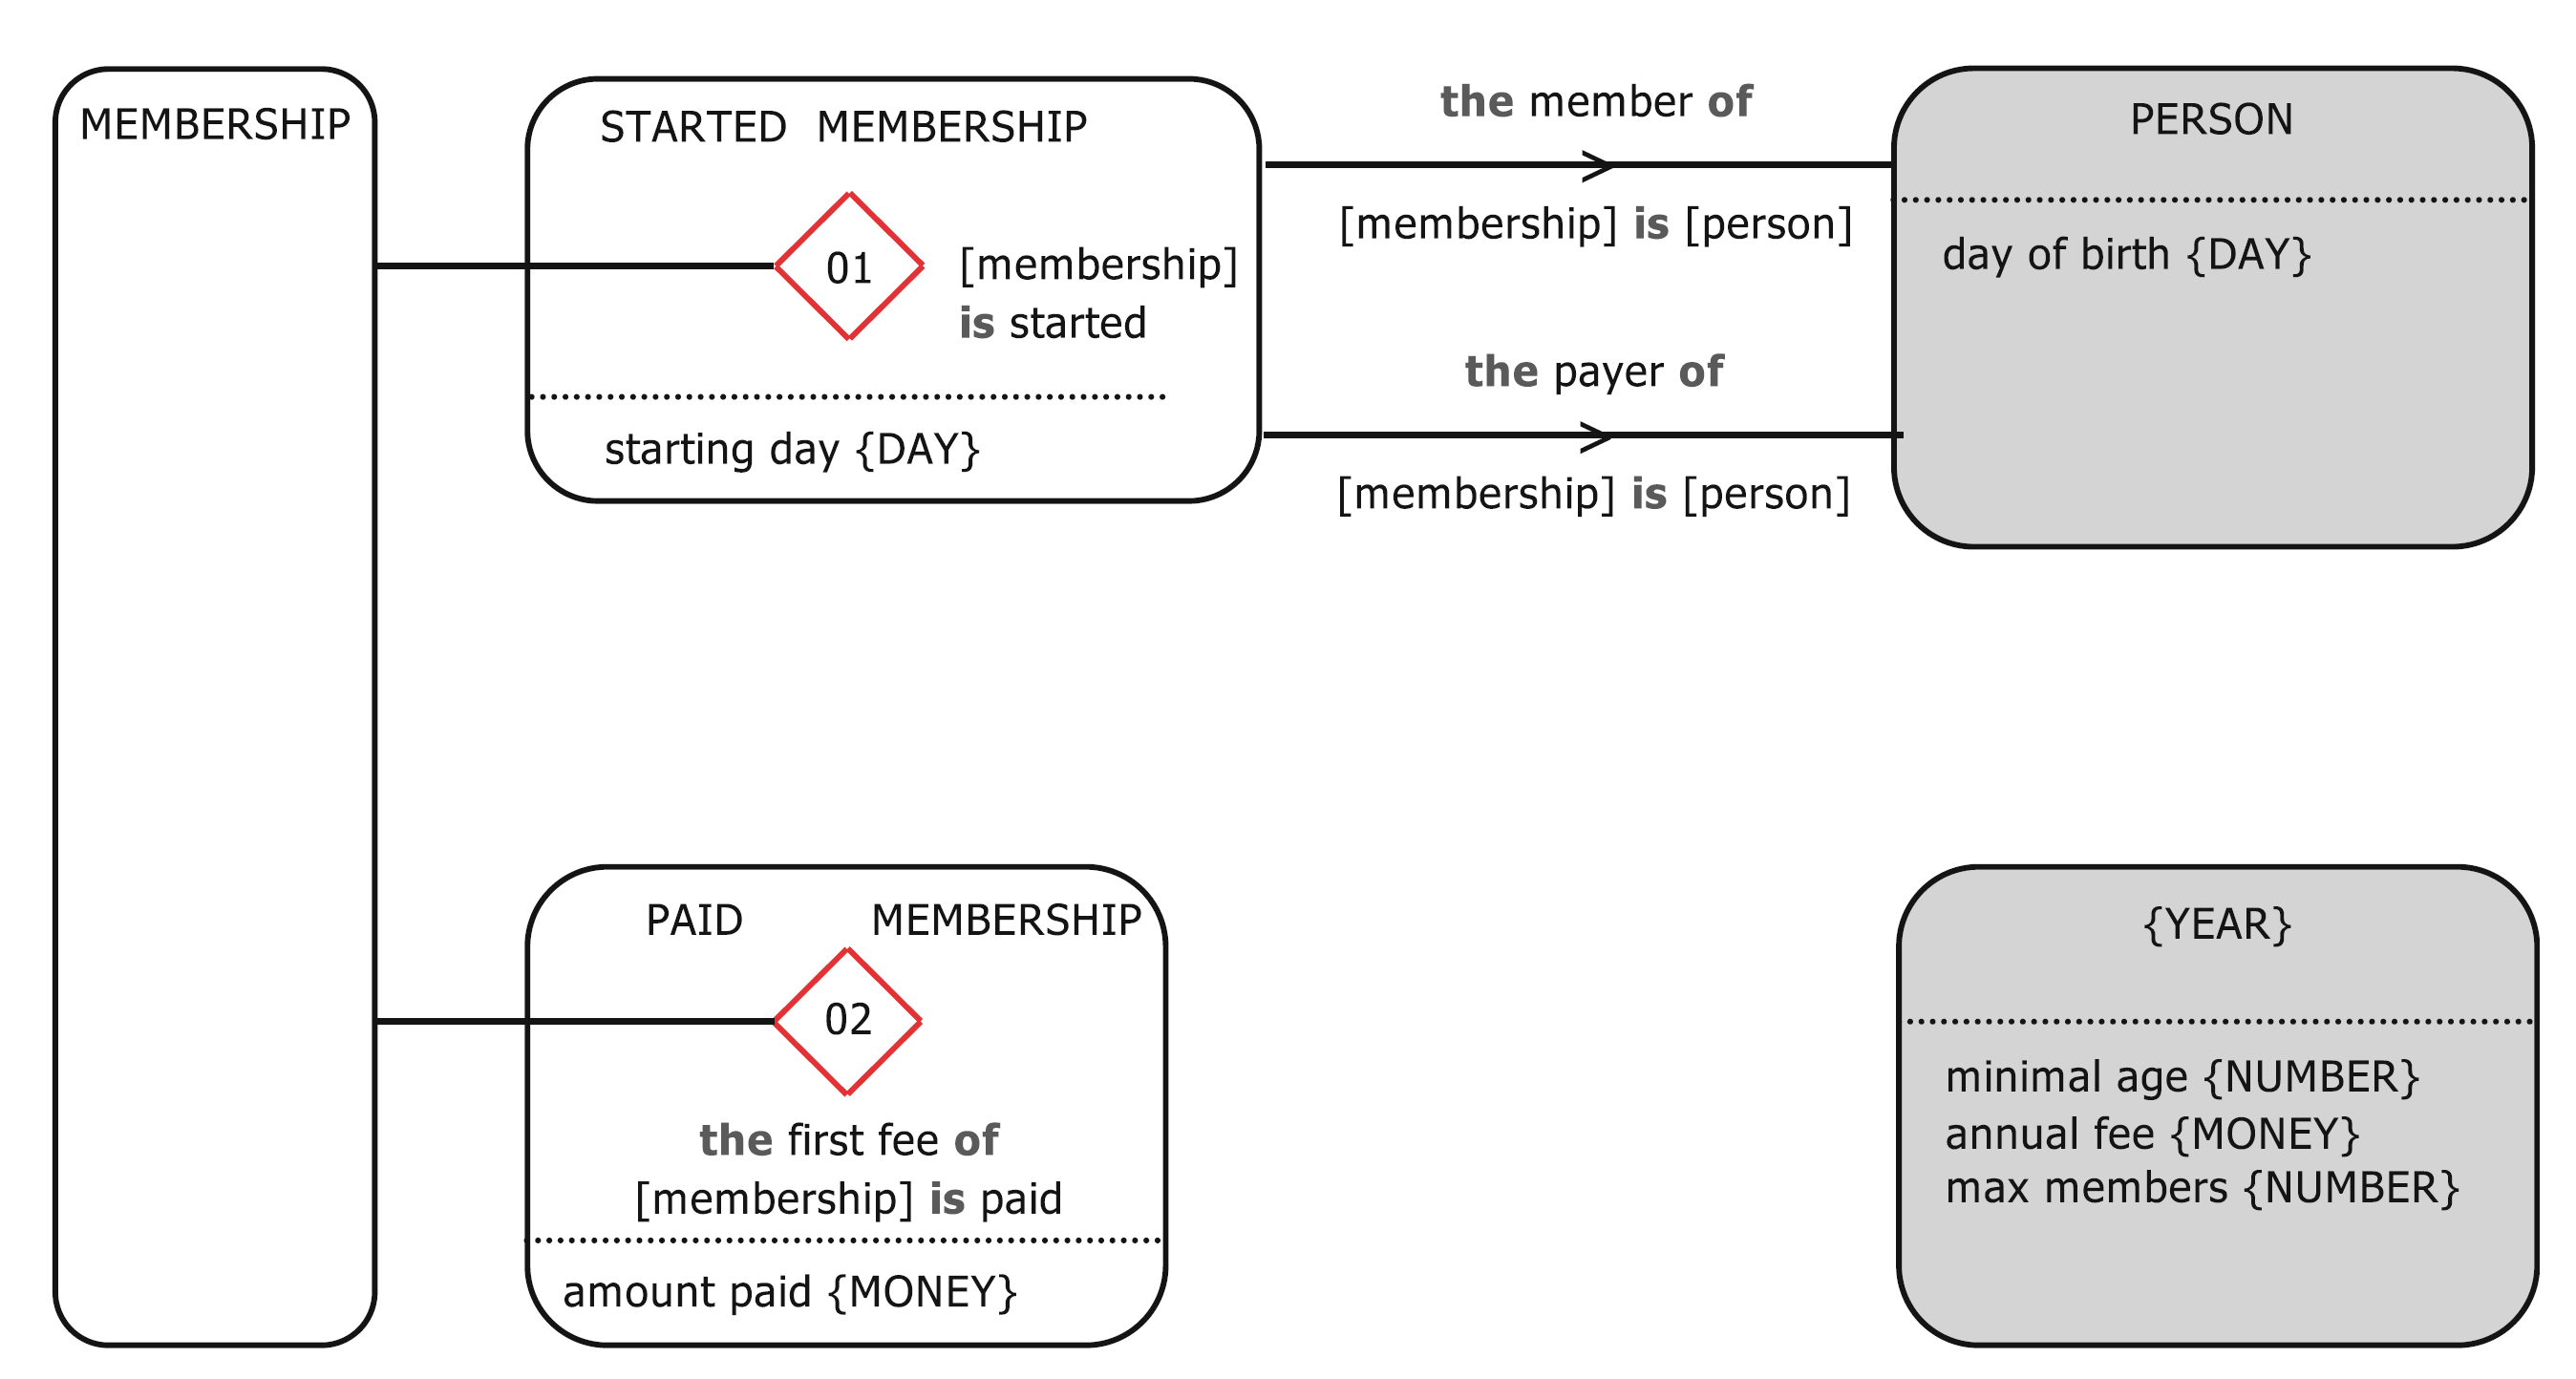
\includegraphics[width=12cm]{pic/VolleyOFD.png}
	\caption{An Object Fact Diagram of Volley~\cite{dietz2020enterprise}}
	\label{fig:ofdModel}
\end{figure}


\section{Summary}

Some comments about the OER analysis belong here. Why were you not able find some responsibilities? What was vaguely defined? Just roast the authors of the assignment (not the teachers :). 

And finally, show how much information is missing in a table~\cref{tab:missing_transaction_steps}. 

\begin{table}[h]\centering
\caption{Missing Transaction Steps}
\label{tab:missing_transaction_steps}
\begin{tabular}{|l||l|l|l|}
\hline
                      & Specified    & Not Specified & Missing Information \\ \hline
\multicolumn{4}{|c|}{Standard Transaction Pattern}                        \\ \hline
Request               & 2           & 0            & 0\%             \\ \hline
Promise               & 1           & 1            & 50\%            \\ \hline
Decline               & 1          & 1           & 50\%             \\ \hline
Declare               & 2           & 0            & 0\%              \\ \hline
Reject                & 0            & 2           & 100\%             \\ \hline
Accept                & 0           & 2            & 100\%            \\ \hline
\textbf{Total}        & \textbf{6} & \textbf{6}  & \textbf{50\%}   \\ \hline
\multicolumn{4}{|c|}{Revokes}                                             \\ \hline
Revoke Request        & 0            & 2           & 100\%             \\ \hline
Revoke Promise        & 0            & 2           & 100\%             \\ \hline
Revoke Declare        & 0            & 2           & 100\%            \\ \hline
Revoke Accept         & 0            & 2           & 100\%             \\ \hline
\textbf{Total}        & \textbf{0}   & \textbf{8} & \textbf{100\%}    \\ \hline
\multicolumn{4}{|c|}{Complete Transaction Pattern}                        \\ \hline
\textbf{Total}        & \textbf{6} & \textbf{14} & \textbf{70\%}    \\ \hline
\end{tabular}

\end{table}